\acresetall


%We will soon embark on a new era of discovery.
%A machine which can observe the universe in a whole new way is about to be
%turned on.
%The significance of this cannot be understated.
%We are about to make history.

%Of course, a drammatic introduction wouldn't be complete without a statement
%on how sentient beings have always gazed at the heavens in wonder.
%We still strive for this understanding and must never let it end.
%The struggles of humankind are too great to let our inspirations fizzle.
%Hope for the future is what sustains us.
%
%Something about Gallileo, Newton, Michelson, Einstein...

We've been making gravitational wave detectors for several years.
The resonant bar detectors of the past have given way to the new
interferometric detectors which have achieved impressive sensitivities
but are soon to be dramatically surpassed
by detectors with a more sophisticated optical layout, including Fabry-Perot
arm cavities, power recycling, and signal extraction.

%Something about detuned signal recycling cavities and resonant enhancement.
%This is it folks. This is the big one...

The next generation of gravitational wave detectors are rapidly coming
online.
Advanced LIGO will be at design sensitivity within a year.
These new detectors will see further, by an order of magnitude over
initial LIGO, this corresponds to a 1000 times greater surveilled volume.
%A thousand times more detector volume.
At this sensitivity, one day of Advanced LIGO observations will surveil a
larger space-time volume than the 2 years of observations with initial LIGO.
%And with the advancements in lock acquisition, we will surpass the entire
%integrated volume of initial LIGO in the blink of an eye.
aLIGO isn't a simple upgrade, it's literally a new detector.
Every component has been ripped out and replaced.
The laser source is new, pumping out a massive
%1.21 jigaWatts
180 Watts of power.
The radiation pressure noise associated with this power will start to
dominate the displacement noise of the new 40kg test masses.
%it will start to dominate even the new 40kg test masses.
From the state of the art coatings technology to the silicate bonded
monolithic fused silica fiber assemblies we have left virtually
%\footnote{with the interesting exception of the output mode cleaner, which
%serves as the readout point for the gravitational wave signal.}
nothing untouched.

%As I am sitting on a plane, writing my thesis, and listening to the soundtrack
%to TRON,
As I am writing this,
the detector in Livingston is already beginning to surpass the
best sensitivity we ever had in initial LIGO. The detector at Hanford will
soon be sealed in it's capsule to embark on a journey into the farthest
reaches of the
universe\footnote{Manufacturing errors in the test mass coatings required a new
set to be installed, delaying the closure of the vacuum system.}.

Reflecting over my time at Syracuse, we have seen the Large Hadron Collider
turn on and confirm the existence of those things we were looking
for\footnote{the Higgs Boson}.
Of course I can't just leave the Higgs Boson as a footnote.
This is what gives matter it's mass and as far as we know we can't have
gravitational waves without mass.
Well, we wouldn't exist without mass either, but that's beside the point...

%My time at Syracuse has brought me great joy.
%I have worked with many from throughout LIGO.

%Of course, my greatest joy comes from my family.
%Without them, I'm not sure I would have ever left my office/lab.
%We have had such a great experience here and made many friends of which we
%will never forget.


%For my children, it is your future that I live for.
%May your own inspirations come with great strength.

From this we begin,
\begin{equation}
F = ma\,.
\end{equation}


\section{Gravitational Waves}

The foundation of Einstein's theory of general relativity is that the motion
of a freely falling body is governed by the local space-time curvature.
This curvature is in turn influenced by the presence of
matter.
% \footnote{matter being stuff that has mass}.
This matter not only curves the space it occupies, but also curves the space
around it.
% in such a way as to result in an acceleration on an object given by,
% \begin{equation}
% a = \frac{GM}{r^2} \;.
% \end{equation}

As matter moves through space, the curvature of space changes.
%Not only is the curvature changing in the space in which the matter is
%moving, it is also changing away from the mass.
Special relativity tells us that information cannot travel faster than the
speed of light.
The information about how the curvature of space is changing must propagate
at finite speed.
From the multipole expansion of the mass distribution, the monopole (which is
the first term) is a scalar quantity that is simply the total
mass of the object.
The second term is, called the 'dipole' is a vector which is the sum of all the
bits of mass multiplied by their position vector from a fixed reference point.
The dipole term is identically the center of mass location times the total mass.
This term can change with time, however the first derivative $mv$ (momentum)
is conserved.
The third term is known as the quadrupole term.
It is this term which has a non zero second derivative that gives rise to a
wave equation.
And the amplitude of this gravitational wave is,
\begin{equation}
h = \frac{2G}{c^4r}\ddot I \;,
\end{equation}
where the unitless term $h$ is the gravitational wave strain.
This strain is the $\frac{\Delta L}{L}$ perturbation on the background
space-time metric that we are looking for.
Gravitational waves stretch space-time in one
direction while squeezing it in the orthogonal direction.



We look for the strain perturbations by measuring the distance between two
freely falling objects we call test masses.
In the simple case of a two test mass detector (one arm of LIGO) we are only
sensitive to half of the signal (assuming optimal orientation).
Since the orthogonal direction is moving in the opposite way, it would be
natural to choose an instrument which measures the difference in length between
two orthogonal directions.
%makes a differential length detector
%a natural choice
And with two orthogonal arms we are sensitive to the full
amplitude of the wave.
It is important to note that this factor of 2 increase in the signal, though
helpful, is not the primary motivation for two arms. 
The big benefit comes from common noise cancellation.
We can cancel out common length noise,
typically dominated by frequency noise
in the two arms because the gravitational
wave will couple directly into the differential degree of freedom in the
detector.
See figure \ref{fig:ligoschematic}.

\begin{figure}
\tikzsetnextfilename{ligoschematic}
\centering
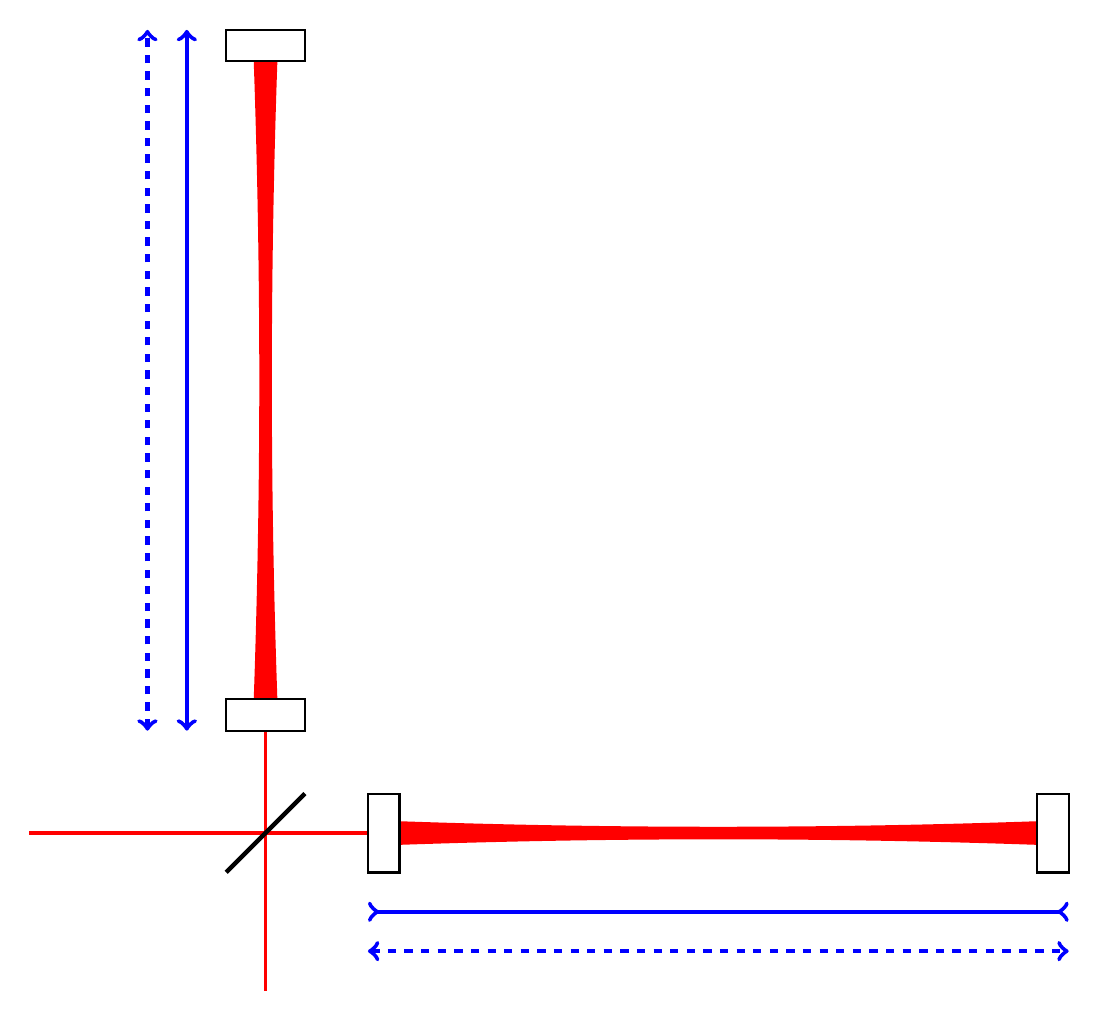
\begin{tikzpicture}
%  \draw[thick,rotate=45] (-1,-0.2) rectangle (1,0.2);
  \draw[very thick,red] (-3,0) -- (1.3,0);
  \draw[very thick,red] (0,0) -- (0,1.3);
  \draw[very thick,red] (0,0) -- (0,-2);
  \fill[red] (1.7,-0.15) arc (92:88:116.048) -- ++(0,0.3) arc (272:268:116.048) -- cycle;
  \fill[red] (-0.15,1.7) arc (-2:2:116.048) -- ++(0.3,0) arc (178:182:116.048) -- cycle;
  \draw[ultra thick] (-0.5,-0.5) -- (0.5,0.5);
  \draw[thick] (1.3,-0.5) rectangle (1.7,0.5);
  \draw[thick] (9.8,-0.5) rectangle (10.2,0.5);
  \draw[thick] (-0.5,1.3) rectangle (0.5,1.7);
  \draw[thick] (-0.5,9.8) rectangle (0.5,10.2);
  \draw[ultra thick,blue,<->] (-1,1.3) -- (-1,10.2);
  \draw[ultra thick,dashed,blue,<->] (-1.5,1.3) -- (-1.5,10.2);
  \draw[ultra thick,blue,>-<] (1.3,-1) -- (10.2,-1);
  \draw[ultra thick,dashed,blue,<->] (1.3,-1.5) -- (10.2,-1.5);
\end{tikzpicture}
\caption[LIGO Schematic]{This schematic shows the layout of a basic
    interferometric gravitational wave detector.
    Each arm of the interferometer is a Fabry-Perot cavity which circulates
    the light in the arms, increasing the response of the detector.
    The blue lines indicate the common (dashed) and differential (solid)
    degrees of freedom.
    The Michelson naturally reads out the differential degree of freedom which
    is free of common noise such as the intensity and frequency noise of the
    laser.
    }
\label{fig:ligoschematic}
\end{figure}


%A pea sized amount of neutron star material has the mass of about 100,000
%locomotives.

%\section{Angular Control Using Optical Traps}

\section{Angular Control}

In order for our instrument to be sensitive to gravitational waves we want
the test masses to swing freely.
Also, since the gravitational wave amplitude is a strain and we are measuring
changes in length, we get better sensitivity with longer arms.
Longer arms, however, also make it more difficult to keep the mirrors pointed
at each other.
An angular control system is necessary for the sensitive alignment of the
instrument.

In Advanced LIGO we use an active feedback control for angular alignment of
the main mirrors\cite{aligowfs}.
%which is discussed in more detail in the angular instability section of our
%theory paper which is provided in \ref{sec:IV}.
Sensing for this feedback is done with a technique known as \ac{wfs}.
The beam entering a cavity is phase modulated to produce sidebands.
The phase modulation is done at a high enough frequency so that almost all
of the sideband beams are reflected.

% \begin{figure}
% \tikzsetnextfilename{sbrefl}
% \centering
% \begin{tikzpicture}
%   \draw[very thick,red,->] (-3,0) -- (0,0) arc (90:-90:0.1) -- +(180:1);
%   \draw[very thick,blue,->] (-3,0.05) -- (0,0.05) arc (90:-90:0.1) -- +(180:1);
%   \draw[very thick,red,->] (0,0) -- (5,0) arc (90:-90:0.1) -- +(180:4.9);
%   \draw[very thick] (0.1,0) arc (180:170:3.75);
%   \draw[very thick] (0.1,0) arc (180:190:3.75);
%   \draw[very thick] (5.1,0) arc (0:10:3.75);
%   \draw[very thick] (5.1,0) arc (0:-10:3.75);
% \end{tikzpicture}
% \caption[Wavefront sensing beam in reflection]{
%   beam reflected from cavity for wavefront sensing.
%   The blue line represents the sideband beam which is promptly reflected from
%   the input mirror.
%   The red line represents the carrier beam.
%   The reflected carrier beam has components reflected from the input and from
%   the output mirrors.
% }
% \label{fig:sbrefl}
% \end{figure}
% 
% \begin{figure}
% \tikzsetnextfilename{sbreflwav}
% \centering
% \begin{tikzpicture}
%   \draw[very thick,red,->] (-3,0) -- (0,0);
%   \draw[very thick,blue,->] (-3,0.05) -- (0,0.05);
%   \draw[very thick,red,->] (0,0) -- (5,0);
%   \draw[very thick] (0.1,0) arc (180:170:3.75);
%   \draw[very thick] (0.1,0) arc (180:190:3.75);
%   \draw[thick,blue] (0,0) arc (180:175:3.85);
%   \draw[thick,blue] (0,0) arc (180:185:3.85);
%   \draw[thick,blue] (-0.2,0) arc (180:175:4.05);
%   \draw[thick,blue] (-0.2,0) arc (180:185:4.05);
%   \draw[thick,blue] (-0.4,0) arc (180:175:4.25);
%   \draw[thick,blue] (-0.4,0) arc (180:185:4.25);
%   \draw[thick,blue] (-0.6,0) arc (180:175:4.45);
%   \draw[thick,blue] (-0.6,0) arc (180:185:4.45);
%   \draw[thick,blue] (-0.8,0) arc (180:175:4.65);
%   \draw[thick,blue] (-0.8,0) arc (180:185:4.65);
%   \draw[thick,red] (0.2,0) arc (180:175:3.65);
%   \draw[thick,red] (0.2,0) arc (180:185:3.65);
%   \draw[thick,red] (0.4,0) arc (180:175:3.45);
%   \draw[thick,red] (0.4,0) arc (180:185:3.45);
%   \draw[thick,red] (0.6,0) arc (180:175:3.25);
%   \draw[thick,red] (0.6,0) arc (180:185:3.25);
%   \draw[thick,red] (-0.1,0) arc (180:175:3.95);
%   \draw[thick,red] (-0.1,0) arc (180:185:3.95);
%   \draw[thick,red] (-0.3,0) arc (180:175:4.15);
%   \draw[thick,red] (-0.3,0) arc (180:185:4.15);
%   \draw[thick,red] (-0.5,0) arc (180:175:4.35);
%   \draw[thick,red] (-0.5,0) arc (180:185:4.35);
%   \draw[very thick] (5.1,0) arc (0:10:3.75);
%   \draw[very thick] (5.1,0) arc (0:-10:3.75);
% \end{tikzpicture}
% \caption[Wavefront sensing beam in reflection]{
%   beam reflected from cavity for wavefront sensing.
%   The blue line represents the sideband beam which is promptly reflected from
%   the input mirror.
%   The red line represents the carrier beam.
%   The reflected carrier beam has components reflected from the input and from
%   the output mirrors.
% }
% \label{fig:sbreflwav}
% \end{figure}
% 
% \begin{figure}
% \tikzsetnextfilename{sbreflang}
% \centering
% \begin{tikzpicture}
%   \draw[very thick,red,->] (-3,0) -- (0,0) arc (90:-90:0.1) -- +(180:2);
%   \draw[very thick,blue,->] (-3,0.05) -- (0,0.05) arc (90:-90:0.1) -- +(180:2);
%   \draw[very thick,red,->] (0.1,0) -- (5,0.2) arc (92.5:-87.5:0.1) -- +(182.5:7);
%   \draw[very thick] (0.1,0) arc (180:170:3.75);
%   \draw[very thick] (0.1,0) arc (180:190:3.75);
%   \draw[very thick] (5.1,0) arc (10:20:3.75);
%   \draw[very thick] (5.1,0) arc (10:0:3.75);
% \end{tikzpicture}
% \caption[Wavefront sensing beam in reflection]{
%   beam reflected from cavity for wavefront sensing.
%   The blue line represents the sideband beam which is promptly reflected from
%   the input mirror.
%   The red line represents the carrier beam.
%   The reflected carrier beam has components reflected from the input and from
%   the output mirrors.
% }
% \label{fig:sbreflang}
% \end{figure}

\newcommand{\bra}[1]{\left\langle #1 \right|}
\newcommand{\ket}[1]{\left| #1 \right\rangle}
\newcommand{\braket}[2]{\left\langle #1 | #2 \right\rangle}
\newcommand{\braopket}[3]{\left\langle #1 \left| #2 \right| #3 \right\rangle}
\begin{figure}
  \centering
  \subfloat[$\mathrm{TEM}_{00}$ mode ($\ket{00}$)]{%
    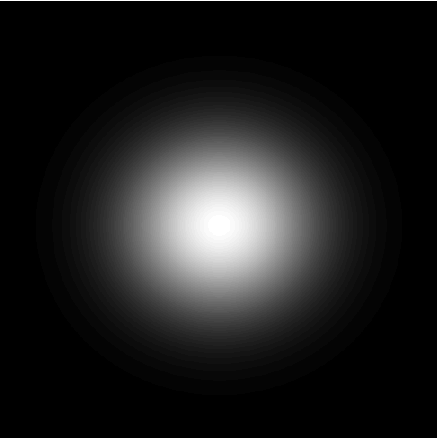
\includegraphics[width=5cm]{./figures/hg00-crop.pdf}
  }
  \subfloat[$\mathrm{TEM}_{01}$ mode ($\ket{10}$)]{%
    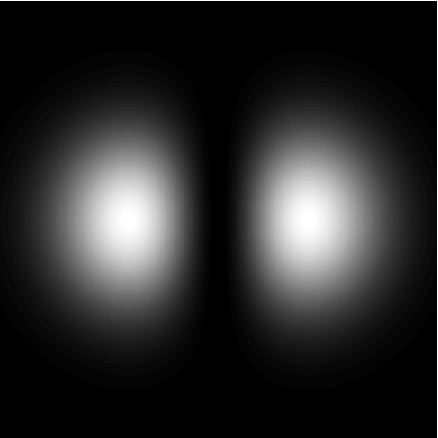
\includegraphics[width=5cm]{./figures/hg01-crop.pdf}
  }
  \subfloat[$\mathrm{TEM}_{10}$ mode ($\ket{01}$)]{%
    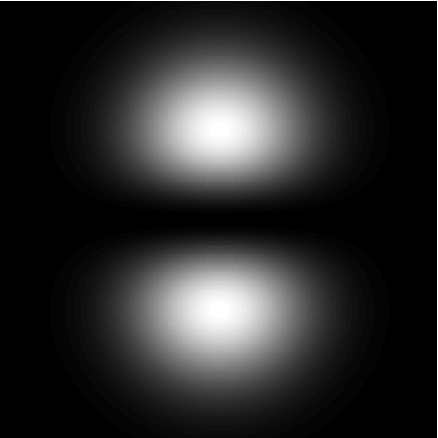
\includegraphics[width=5cm]{./figures/hg10-crop.pdf}
  }
  \caption[Hermite-Gaussian Modes]{Hermite-Gauss modes. The first three
    transverse electro magnetic modes from Hermite-Gauss decomposition are
    depicted here.
    These images indicate the power density across the transverse
    dimensions.
    There is one first order mode for each transverse dimension.
    The first order modes are odd functions in field amplitude along the
    respective dimension.
    }
  \label{fig:hgmodes}
\end{figure}

\begin{figure}
  \centering
  \subfloat[both mirrors aligned to incoming beam\label{fig:sbreflanga}]{%
  \tikzsetnextfilename{sbreflwava}
  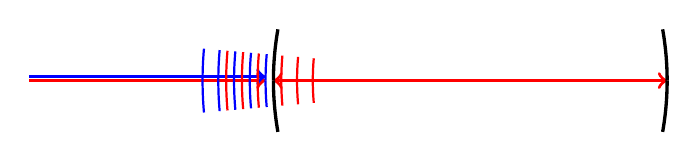
\begin{tikzpicture}
    \draw[very thick,red,->] (-3,0) -- (0,0);
    \draw[very thick,blue,->] (-3,0.05) -- (0,0.05);
    \draw[very thick,red,->] (2.6,0) -- (5.1,0);
    \draw[very thick,red,->] (2.6,0) -- (0.1,0);
    \draw[very thick] (0.1,0) arc (180:170:3.75);
    \draw[very thick] (0.1,0) arc (180:190:3.75);
    \draw[thick,blue] (0,0) arc (180:175:3.85);
    \draw[thick,blue] (0,0) arc (180:185:3.85);
    \draw[thick,blue] (-0.2,0) arc (180:175:4.05);
    \draw[thick,blue] (-0.2,0) arc (180:185:4.05);
    \draw[thick,blue] (-0.4,0) arc (180:175:4.25);
    \draw[thick,blue] (-0.4,0) arc (180:185:4.25);
    \draw[thick,blue] (-0.6,0) arc (180:175:4.45);
    \draw[thick,blue] (-0.6,0) arc (180:185:4.45);
    \draw[thick,blue] (-0.8,0) arc (180:175:4.65);
    \draw[thick,blue] (-0.8,0) arc (180:185:4.65);
    \draw[thick,red] (0.2,0) arc (180:175:3.65);
    \draw[thick,red] (0.2,0) arc (180:185:3.65);
    \draw[thick,red] (0.4,0) arc (180:175:3.45);
    \draw[thick,red] (0.4,0) arc (180:185:3.45);
    \draw[thick,red] (0.6,0) arc (180:175:3.25);
    \draw[thick,red] (0.6,0) arc (180:185:3.25);
    \draw[thick,red] (-0.1,0) arc (180:175:3.95);
    \draw[thick,red] (-0.1,0) arc (180:185:3.95);
    \draw[thick,red] (-0.3,0) arc (180:175:4.15);
    \draw[thick,red] (-0.3,0) arc (180:185:4.15);
    \draw[thick,red] (-0.5,0) arc (180:175:4.35);
    \draw[thick,red] (-0.5,0) arc (180:185:4.35);
    \draw[very thick] (5.1,0) arc (0:10:3.75);
    \draw[very thick] (5.1,0) arc (0:-10:3.75);
  \end{tikzpicture}
  }

  \subfloat[output mirror misaligned to incoming beam\label{fig:sbreflangb}]{%
  \tikzsetnextfilename{sbreflwavb}
  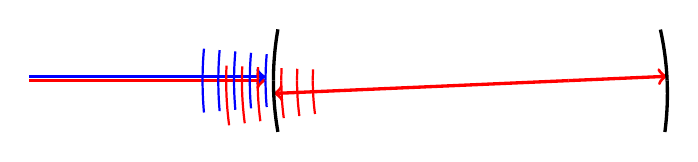
\begin{tikzpicture}
    \draw[very thick,red,->] (-3,0) -- (0,0);
    \draw[very thick,blue,->] (-3,0.05) -- (0,0.05);
    \draw[very thick,red,->] (3.85,0) -- +(2.5:1.25);
    \draw[very thick,red,->] (3.85,0) -- +(182.5:3.75);
    \draw[very thick] (0.1,0) arc (180:170:3.75);
    \draw[very thick] (0.1,0) arc (180:190:3.75);
    \draw[thick,blue] (0,0) arc (180:175:3.85);
    \draw[thick,blue] (0,0) arc (180:185:3.85);
    \draw[thick,blue] (-0.2,0) arc (180:175:4.05);
    \draw[thick,blue] (-0.2,0) arc (180:185:4.05);
    \draw[thick,blue] (-0.4,0) arc (180:175:4.25);
    \draw[thick,blue] (-0.4,0) arc (180:185:4.25);
    \draw[thick,blue] (-0.6,0) arc (180:175:4.45);
    \draw[thick,blue] (-0.6,0) arc (180:185:4.45);
    \draw[thick,blue] (-0.8,0) arc (180:175:4.65);
    \draw[thick,blue] (-0.8,0) arc (180:185:4.65);
    \draw[thick,red] (0.2,0) arc (180:177.5:3.65);
    \draw[thick,red] (0.2,0) arc (180:187.5:3.65);
    \draw[thick,red] (0.4,0) arc (180:177.5:3.45);
    \draw[thick,red] (0.4,0) arc (180:187.5:3.45);
    \draw[thick,red] (0.6,0) arc (180:177.5:3.25);
    \draw[thick,red] (0.6,0) arc (180:187.5:3.25);
    \draw[thick,red] (-0.1,0) arc (180:177.5:3.95);
    \draw[thick,red] (-0.1,0) arc (180:187.5:3.95);
    \draw[thick,red] (-0.3,0) arc (180:177.5:4.15);
    \draw[thick,red] (-0.3,0) arc (180:187.5:4.15);
    \draw[thick,red] (-0.5,0) arc (180:177.5:4.35);
    \draw[thick,red] (-0.5,0) arc (180:187.5:4.35);
%   \draw[very thick] (5.1,0) arc (0:10:3.75);
%   \draw[very thick] (5.1,0) arc (0:-10:3.75);
    \draw[very thick] (5.1,0) arc (2.5:12.5:3.75);
    \draw[very thick] (5.1,0) arc (2.5:-7.5:3.75);
  \end{tikzpicture}
  }
  \caption[Wavefront sensing beam in reflection]{
    beam reflected from cavity for wavefront sensing.
    The input beam to the cavity is from the left.
    Blue represents the sideband beams which are promptly reflected from the
    input mirror.
    Red represents the carrier beam which resonates in the cavity.
%    The blue line represents the sideband beam which is promptly reflected from
%    the input mirror.
%    The red line represents the carrier beam.
%    The reflected carrier beam has components reflected from the input and from
%    the output mirrors.
    The curves represent the wavefronts of each as they are added together in
    reflection.
    Misalignment of a mirror causes a
    transverse offset between the reflected carrier beam and the reflected
    subcarrier beam.
    So, in the transverse mode basis of the reflected sidebands, the reflected
    carrier gains higher order mode content.
    This higher order mode content contains the alignment information which is
    detected with the wavefront sensor.
  }
  \label{fig:sbreflang}
\end{figure}


Wavefront sensing works by beating the carrier beam reflected from the cavity
against the reflected sidebands.
Any misalignment results in a 1st order mode component of the reflected carrier
beam relative to the reflected sidebands.
This effect is shown in figure \ref{fig:sbreflang}.
If we were to then integrate over the transverse dimensions using a photodiode,
the beat signal would produce no amplitude since we are beating together
orthogonal transverse modes.
We can defeat this by splitting the photodiode in two and measuring the
difference between the two sides.

I will illustrate this effect using bra-ket notation.
Keeping things to first order, the reflected carrier beam is composed of the
$\mathrm{TEM}_{00}$ mode with a small amount of the $\mathrm{TEM}_{10}$ mode,
\begin{align}
  \left| \mathrm{CC} \right\rangle &\approx \left| 00 \right\rangle + \eta
    \left| 10 \right\rangle \\
  &= \left| 00 \right\rangle + \eta \left| 00 \right\rangle \frac{2x}{w(z)}
    e^{i\Psi(z)} \; .
\end{align}
The $\mathrm{TEM}_{00}$ mode from the sidebands looks like,
\begin{align}
  \left| \mathrm{SB} \right\rangle &= \left| 00 \right\rangle \cos
    \Omega t \; .
\end{align}
The combined beam in reflection looks like,
\begin{equation}
  \left| \mathrm{REFL} \right\rangle = \left| \mathrm{CC} \right\rangle +
    \left| \mathrm{SB} \right\rangle \; .
\end{equation}

Now, we apply our sensing operator, $\mathrm{PD}$. If $\mathrm{PD}$ is simply
a single photodiode, we get,
\begin{align}
  \left\langle \mathrm{REFL} \left| \mathrm{PD} \right| \mathrm{REFL}
  \right\rangle &= \left\langle 00 | 00 \right\rangle
    \left( 1 + \cos \Omega t \right)^2 +
    2\eta \braket{00}{10} \left(1 + \cos \Omega t \right) +
    \eta^2 \braket{10}{10}
\end{align}
The term which is first order in $\Omega$ will vanish due to orthonormality.
We can defeat this by splitting our photodiode in two and subtracting one side
from the other.
% Then, the $\ket{10}$ field changes from odd to even and the
Now, the integral $\braopket{00}{\mathrm{PD}}{10}$ is no longer zero.
If the photodiode is perfectly aligned with the transverse mode basis,
the integrals $\braopket{00}{\mathrm{PD}}{00}$ and
$\braopket{10}{\mathrm{PD}}{10}$ become zero.

%We will demodulate with the $\Omega$ local oscillator signal. So, with
%$\mathrm{PD}$ as our sensing operator 

%Adding the two beams and then integrating the power across a photodiode gives
%us,
%\begin{align}
%  \left| \mathrm{REFL} \right\rangle &= \left| 00 \right\rangle
%    \left( \cos \Omega t + \frac{2x}{w(z)} e^{i \Psi (z)} \right)^2 \; .
%\end{align}

%%%%%%
% The beat signal is demodulated to give the error signal.

The non-zero beat signal is then demodulated to give us the error signal.


%%%%%%
% The gouy phase allows for an additional degree of freedom in the signal.

From the longitudinal dimension of the wave, we get an additional phase degree
of freedom. There is a Gouy phase term which depends on the distance from the waist
of the beam. The Gouy phase, $\Psi(z)$, is defined by
\begin{align*}
  \tan{\Psi(z)} = z/z_R \;,
\end{align*}
where $z_R$ is the Rayleigh range which is defined as the distance from the beam
waist to the point where the beam radius increases by $\sqrt{2}$.

%%%%%%
% The input test mass and end test mass are at different gouy phases, allowing
% us to sense the alignment degree of freedom for each mirror.

Since the input test mass and end test mass are at different Gouy phases
their misalignment affects a different linear combination of quadratures of the
beam.

%%%%%%
% The idea can be applied to the y-dimension as well to give the two alignment
% degrees of freedom (pitch and yaw)

Splitting the photodiode into four quadrants gives us sensitivity to two
alignment degrees of freedom.

%%%%%%
%
%

We use two quadrant photodiodes for sensing the four angular degrees
of freedom of the two cavity mirrors.
The two \ac{qpd}s are placed in reflection at different distances from the
input mirror for sensing the different Gouy phases.
Then we can transform the four degrees of freedom of the sensor output to the
four degrees of freedom of the mirror alignments.

%This is picked up in a RF quadrant photodiode and demodulated with the local
%oscillator for the sidebands placed on the beam producing a \ac{pdh}
%style error signal for pitch and yaw.


\subsection{Limitations}

%Angular control is necessary to stabilize the Sidles-Sigg instability
%\cite{2006PhLA..354..167S}.

%%%%%%
% There are limitations to this approach which ultimately amount to adding
% noise into the sensitive band of the detector
%
There are limitations to this approach which will ultimately add
noise into the sensitive band of the detector.
This noise comes from the alignment sensing which gets fed back to the
alignment actuators and couples into the gravitational wave strain signal.
% A couple of important limitations come from this technique.

The coupling of angular motion to gravitational wave strain occurs due to
misalignment of the beam on the test masses as well as unbalanced actuation
on the test masses.

%First, we need some
%light to make this work. At the light port there is plenty, but at the dark
%port we need all of the light we can get for the DC readout where we get the
%gravitational wave signal from.
%The feedback can easily be limited by sensing noise since there is very little
%light to work with.

%The second limitation is that for angular stabilization
The ability to attenuate the sensing signal is limited by the fact that
we need to control above the hard mode frequency of the Sidles-Sigg instability
\cite{2006PhLA..354..167S}
which,
for Advanced LIGO at high power, is at about 6 Hz.
We need a sharp cutoff in the feedback below 10Hz in order to not introduce
sensing noise in the sensitive band of LIGO.
There is very little room to attenuate the sensing noise sufficiently above 10
Hz while keeping a stable feedback loop with a unity gain frequency above 6 Hz.

% The technique just described is known as \ac{wfs} and has been a system from initial
% \ac{ligo} and carried over to \ac{aligo}.

As power is increased, the sensing noise from \ac{wfs} will contribute more
to the interferometer noise budget due to the necessary feedback control
requirements.

The \ac{wfs} noise contribution will actually increase at a higher rate
than the contribution
from radiation pressure noise, assuming the control loop has a steep cutoff
above the unity gain frequency.
If we take the sensing noise from \ac{wfs} as constant, the frequency of the
hard mode of the angular instability will increase with $\sqrt{\mathrm{P}}$.
The control bandwith must then also increase at the same rate.
If we also increase the cutoff frequency by $\sqrt{\mathrm{P}}$, the noise
contribution from frequencies above the cutoff will then increase by
$\sqrt{\mathrm{P}^{n}}$, where $n$ is the cutoff rate (feedback open loop goes as
$f^{-n}$).

Without changing power ratios for the \ac{wfs}, the situation is improved a
little.
If we allow the power incident on the \ac{wfs} sensors to increase with the
circulating power in the interferometer, the \ac{wfs} sensing noise will
decrease by $\sqrt{\mathrm{P}}$.
The noise contribution from \ac{wfs} will then increase by
$\sqrt{\mathrm{P}^{n-1}}$ instead of $\sqrt{\mathrm{P}^{n}}$.

At some point, as we push for better sensitivity in the low frequency regime,
there will be a tradeoff between going to higher power in the
interferometer and reducing \ac{wfs} sensing noise coupling to the gravitational
wave strain measurement at low frequencies.
% As power is increased, the frequency of the hard mode of the angular
% instability increases by $\sqrt{\mathrm{P}}$.
% The sensing noise contribution must also increase by $\sqrt{\mathrm{P}}$
% where the feedback transfer function falls off as $1/f$.
% Where the feedback has a steep cutoff, $1/f^\mathrm{n}$, the sensing noise
% contribution must increase by $\sqrt{\mathrm{P^n}}$.
In the region where the noise contribution from \ac{wfs} increases by
$\sqrt{\mathrm{P}^{n-1}}$,
the radiation pressure noise increases by $\sqrt{\mathrm{P}}$.
If the cutoff falls steeper than $f^{-2}$ the \ac{wfs} noise will eventually overtake the radiation pressure noise as the laser power increases.

%It is basically a \ac{pdh} lock with quadrant photo-diodes measuring
%the differential \ac{pdh} signal from opposite quadrants of the photo-diode.

